%%%%%%%%%%%%%%%%%%%%%%%%%%%%%%%%%%%%%%%%%%%%%%%%%%%%%%
%
% This file defines the style for your report
% You don't need to edit it any more, if not to change the authors name.
%
% Search below for the keyword:   GROUP
% insert your group number
%
% Search below for the keyword:   AUTHORS
% insert the name of the authors
%
% If you want to compile your document you have TWO ways
% depending on the fact that 
% 	1) you have inserted only postscript images in your .tex file 
%		---> then go to MODE 1
%	2) you have inserted other kind of images (jpg, pdf, ...) in your .tex file
%		---> then go to MODE 2
%
% MODE 1 
% Type:
% 	latex homebook.tex
%
% If the compilation runs successfully and you want to see the results type:
% 	xdvi homebook.dvi &
% and use the menus to go through the document
%
% If you want to create a pdf type:
% 	dvipdfm homebook.dvi
%
% a homebook.pdf file is created
% you can see it using the command:
% 	acroread homebook.pdf &
%
%
% MODE 2
% Type:
%	pdflatex homebook.tex
%
% If the compilation runs successfully you directly have the pdf file
% and you can see it using the command:
%       acroread homebook.pdf &
%
% 
%%%%%%%%%%%%%%%%%%%%%%%%%%%%%%%%%%%%%%%%%%%%%%%%%%%%%%

\documentclass[10pt,  english, makeidx, a4paper, titlepage, oneside]{book}
\usepackage{babel}
\usepackage{fancyhdr}
\usepackage{makeidx}
\usepackage{titlesec}
\usepackage{listings}
\usepackage{booktabs}

\newenvironment{listato}{\footnotesize}{\normalsize }

%\pagestyle{empty}

\textwidth 15.5cm
\textheight 23cm
\topmargin -1cm
\oddsidemargin -0.5cm
\linespread{1.1}
\setlength\parindent{0cm}
\setlength{\parskip}{6pt}

\pagestyle{fancy}
\lhead{}
\chead{Microelectronic Systems}
\lfoot{}
\cfoot{}
\rfoot{}
\rhead{\thepage}

\usepackage{graphicx}
\usepackage{amsmath}
\usepackage{amsfonts}
\usepackage{amsthm}
\usepackage{amssymb}
%\oddsidemargin -1.1cm
\usepackage{graphicx}
\usepackage{caption}
\usepackage{float}
\usepackage{amsmath}
\usepackage{amssymb}
\usepackage{amsfonts}
\usepackage{amsthm}
%\usepackage{subscript}
\usepackage{empheq}
\usepackage{verbatim}
\usepackage{fancyvrb}

\lstdefinelanguage{VHDL}{morekeywords={library,use,all,entity,generic, is,port,in,out,end,architecture,of,begin,and,if,then,else,elsif,process},morecomment=[l]--}

\lstdefinestyle{vhdl}{language = VHDL, basicstyle = \ttfamily, keywordstyle = \color{keyword}\bfseries, commentstyle = \color{comment}}

\titleformat{\chapter}[display]
{\normalfont\Large\filcenter\sffamily}
{\titlerule[0.5pt]%
\vspace{1pt}
\titlerule
\vspace{1pc}
\LARGE\MakeUppercase{\chaptertitlename} \thechapter
}
{1pc}
{\titlerule
\vspace{1pc}
\Huge}

\makeindex

\begin{document}

\frontmatter
\begin{titlepage}
\vspace{0cm}
\centerline{

\includegraphics[width=3cm]{./logopoli}} 
\vspace{0.5cm}
\centerline{\LARGE Politecnico di Torino}
\vspace{2.5cm}
\centerline{\huge\sf Microelectronic Systems}
\vspace{1cm}
\centerline{\Huge\sf DLX Microprocessor: Design \& Development}
\bigskip
\centerline{\huge\sf Final Project Report}
\vspace{2cm}
\centerline{\Large Master degree in Electronics Engineering}
\bigskip
\centerline{\Large Master degree in Computer Engineering}
\vspace{4.5cm}
%%%%%%%%%%%%%%%%%%%%%%%%%%%%%%%%%%%%%%%%%%%%%%%%%%%%%%
%
\centerline{\large Referents: Prof. Mariagrazia Graziano, Giovanna Turvani}
\bigskip
\vspace{1cm}
%
%%%%%%%%%%%%%%%%%%%%%%%%%%%%%%%%%%%%%%%%%%%%%%%%%%%%%%
% GROUP
% Change the name of your group below
%
\centerline{\large Authors: Group 52}
\bigskip
%
%%%%%%%%%%%%%%%%%%%%%%%%%%%%%%%%%%%%%%%%%%%%%%%%%%%%%%
% AUTHORS
% Change the name of the Group participants here
%
\centerline{\large name1, name2}
%
%%%%%%%%%%%%%%%%%%%%%%%%%%%%%%%%%%%%%%%%%%%%%%%%%%%%%%
\vspace{2cm}
\centerline{\large \today}
\end{titlepage}

\tableofcontents

\mainmatter
%%%%%%%%%%%%%%%%%%%%%%%%%%%%%%%%%%%%%%%%%%%%%%%%%%%%%%
%    
% HERE IS WHERE YOU INCLUDE YOUR CHAPTERS
%
%%%%%%%%%%%%%%%%%%%%%%%%%%%%%%%%%%%%%%%%%%%%%%%%%%%%%
% This will help you in writing your homebook
% Remember that the character % is a comment in latex
%
% chapter 1
\chapter{Adders}
\label{chap1}

%%%%%%%%%%%%%%%%%%%%%%%%%%%%%%%%%%%%%%%%%%%%%%%%%%%%%%%%%%%
% you can organize a chapter using sections -> \section{Simulating an inverter}
% or subsections -> \subsection{simulating a particular type of inverter}

%%%%%%   First section

\section{Full Adder}

Adders are one of the most used digital components in computer processors. In general an adder is a digital circuit that implements the sum of two numbers expressed on N bits.\\
In particular, a full adder (FA) is characterized by three inputs and two outputs. If we consider a one-bit full adder, the three inputs are the two numbers to sum and the input carry. The outputs are the sum and the output carry. A schematic diagram of a one-bit full adder is shown in figure \ref{fig:fa}-A. % here is the reference to the figure below

% Below is shown how you can insert a figure. If you give a label to the figure, you can refer to the figure using \ref{figure_label} as shown above. 

	\begin{figure}[ht]
	\centering
	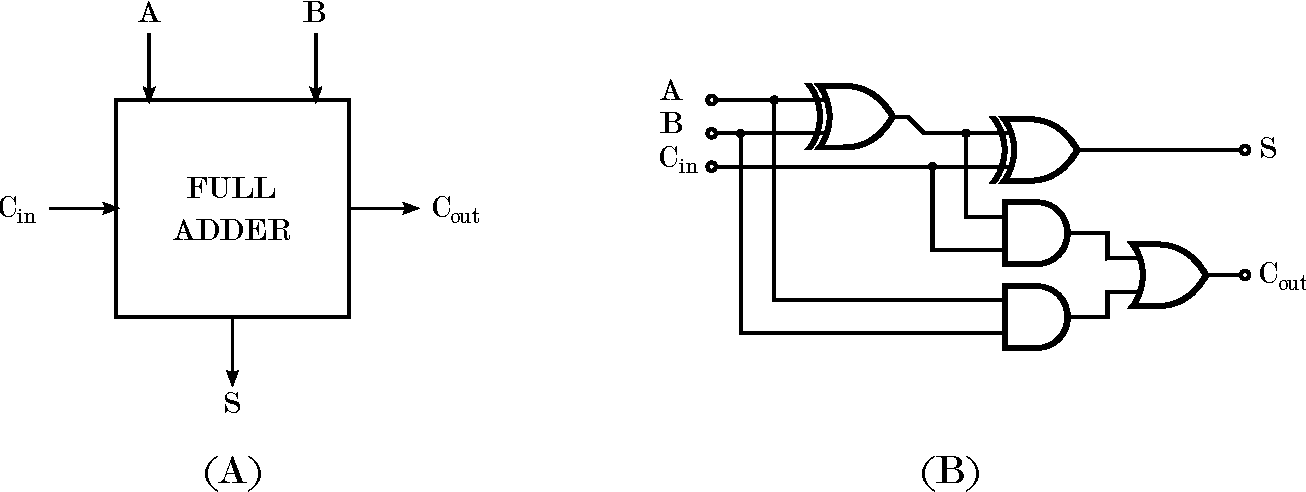
\includegraphics[width=\textwidth]{chapters/figures/fa} 
	\caption{(A) Schematic symbol of a 1-bit full adder. A and B are the operands, Cin is the carry-in while Cout and S are the carry-out and the sum, respectively. (B) Logic diagram of the 1-bit full adder.}
	\label{fig:fa}  % here is the figure label
	\end{figure}

The truth table of the one-bit full adder is shown in table \ref{tab:1}. % here is the reference to the table below

% Below is an example of how to create a simple table. You can create a reference (using \ref{table_label}) to tables too if you give them a label.

	\begin{table}[ht]
	\centering
	\begin{tabular}{ccc}
	\toprule
	A B Cin & S & Cout\\
	\midrule
	0 0 0 & 0 & 0\\
	1 0 0 & 1 & 0\\
	0 1 0 & 1 & 0\\
	1 1 0 & 0 & 1\\
	0 0 1 & 1 & 0\\
	1 0 1 & 0 & 1\\
	0 1 1 & 0 & 1\\
	1 1 1 & 1 & 1\\
	\bottomrule
	\end{tabular}
	\caption{Truth table of a 1-bit full adder.}
	\label{tab:1} % here is the table label
	\end{table}
	
From the truth table we can easily derive the logic equations that describe the full adder:

% Below is an example of how to write equations.

	\begin{equation}
	S = A \oplus B \oplus C_{in}
	\label{eq:1}
	\end{equation}

	\begin{equation}
	C_{out} = AB + C_{in}( A \oplus B)
	\label{eq:2}
	\end{equation}
	
\subsection{Area and power estimation}

A simple Bash script has been written to automatise the calculus of area and power starting from the layout of the circuit. The script takes in input the SVG (which is the primary Inkscape's format) description of the layout and it extracts all the necessary information. The output of the script is a .txt file containing different data.\\
The output text file of the full adder is reported below.

\verbatiminput{chapters/files/planar_FA_area_power.txt}  

% The command \verbatiminput allows you to import the text (e.g, some code or the output resulting from running a program or a script) written in a file.
% You can also include some text in this way:
%	\begin{verbatim}
%		text here
%	\end{verbatim}

% Below is shown how to create an itemize. An alternative to itemize is enumerate that allows you to generate a numbered list. It is used in the same way as itemize:
%	\begin{enumerate}
%		\item bla1
%		\item bla2
%		\item bla3
%	\end{enumerate}

To summarize, the planar full adder is characterized by:
\begin{itemize}
\item Delay = 3 clock cycles;
\item Area = $2.7\ \mu m^2$;
\item Power = $10.53\ \mu W$.
\end{itemize}
	
\section{Ripple Carry Adder}

A Ripple-carry adder (RCA) is a more complex adder composed by a cascade of more full adders. It is used to add N-bit numbers and its name derives from the fact that the carry propagates from a full adder to the next one.\\
\dots \dots \dots \\
\dots \dots \\
\dots
\chapter{Introduction}
\label{chap1}

% introduzione al nostro dlx con le sue caratteristiche: istruzioni implementate, pipelined con quanti stage, stalli, forwarding etc.

\section{Specifications}


\chapter{Functional schema}

% sezione velocemente descrittiva del datapath
\section{Datapath}

% schema del datapath, possibilmente numerato 
\begin{figure}[ht]
	\centering
	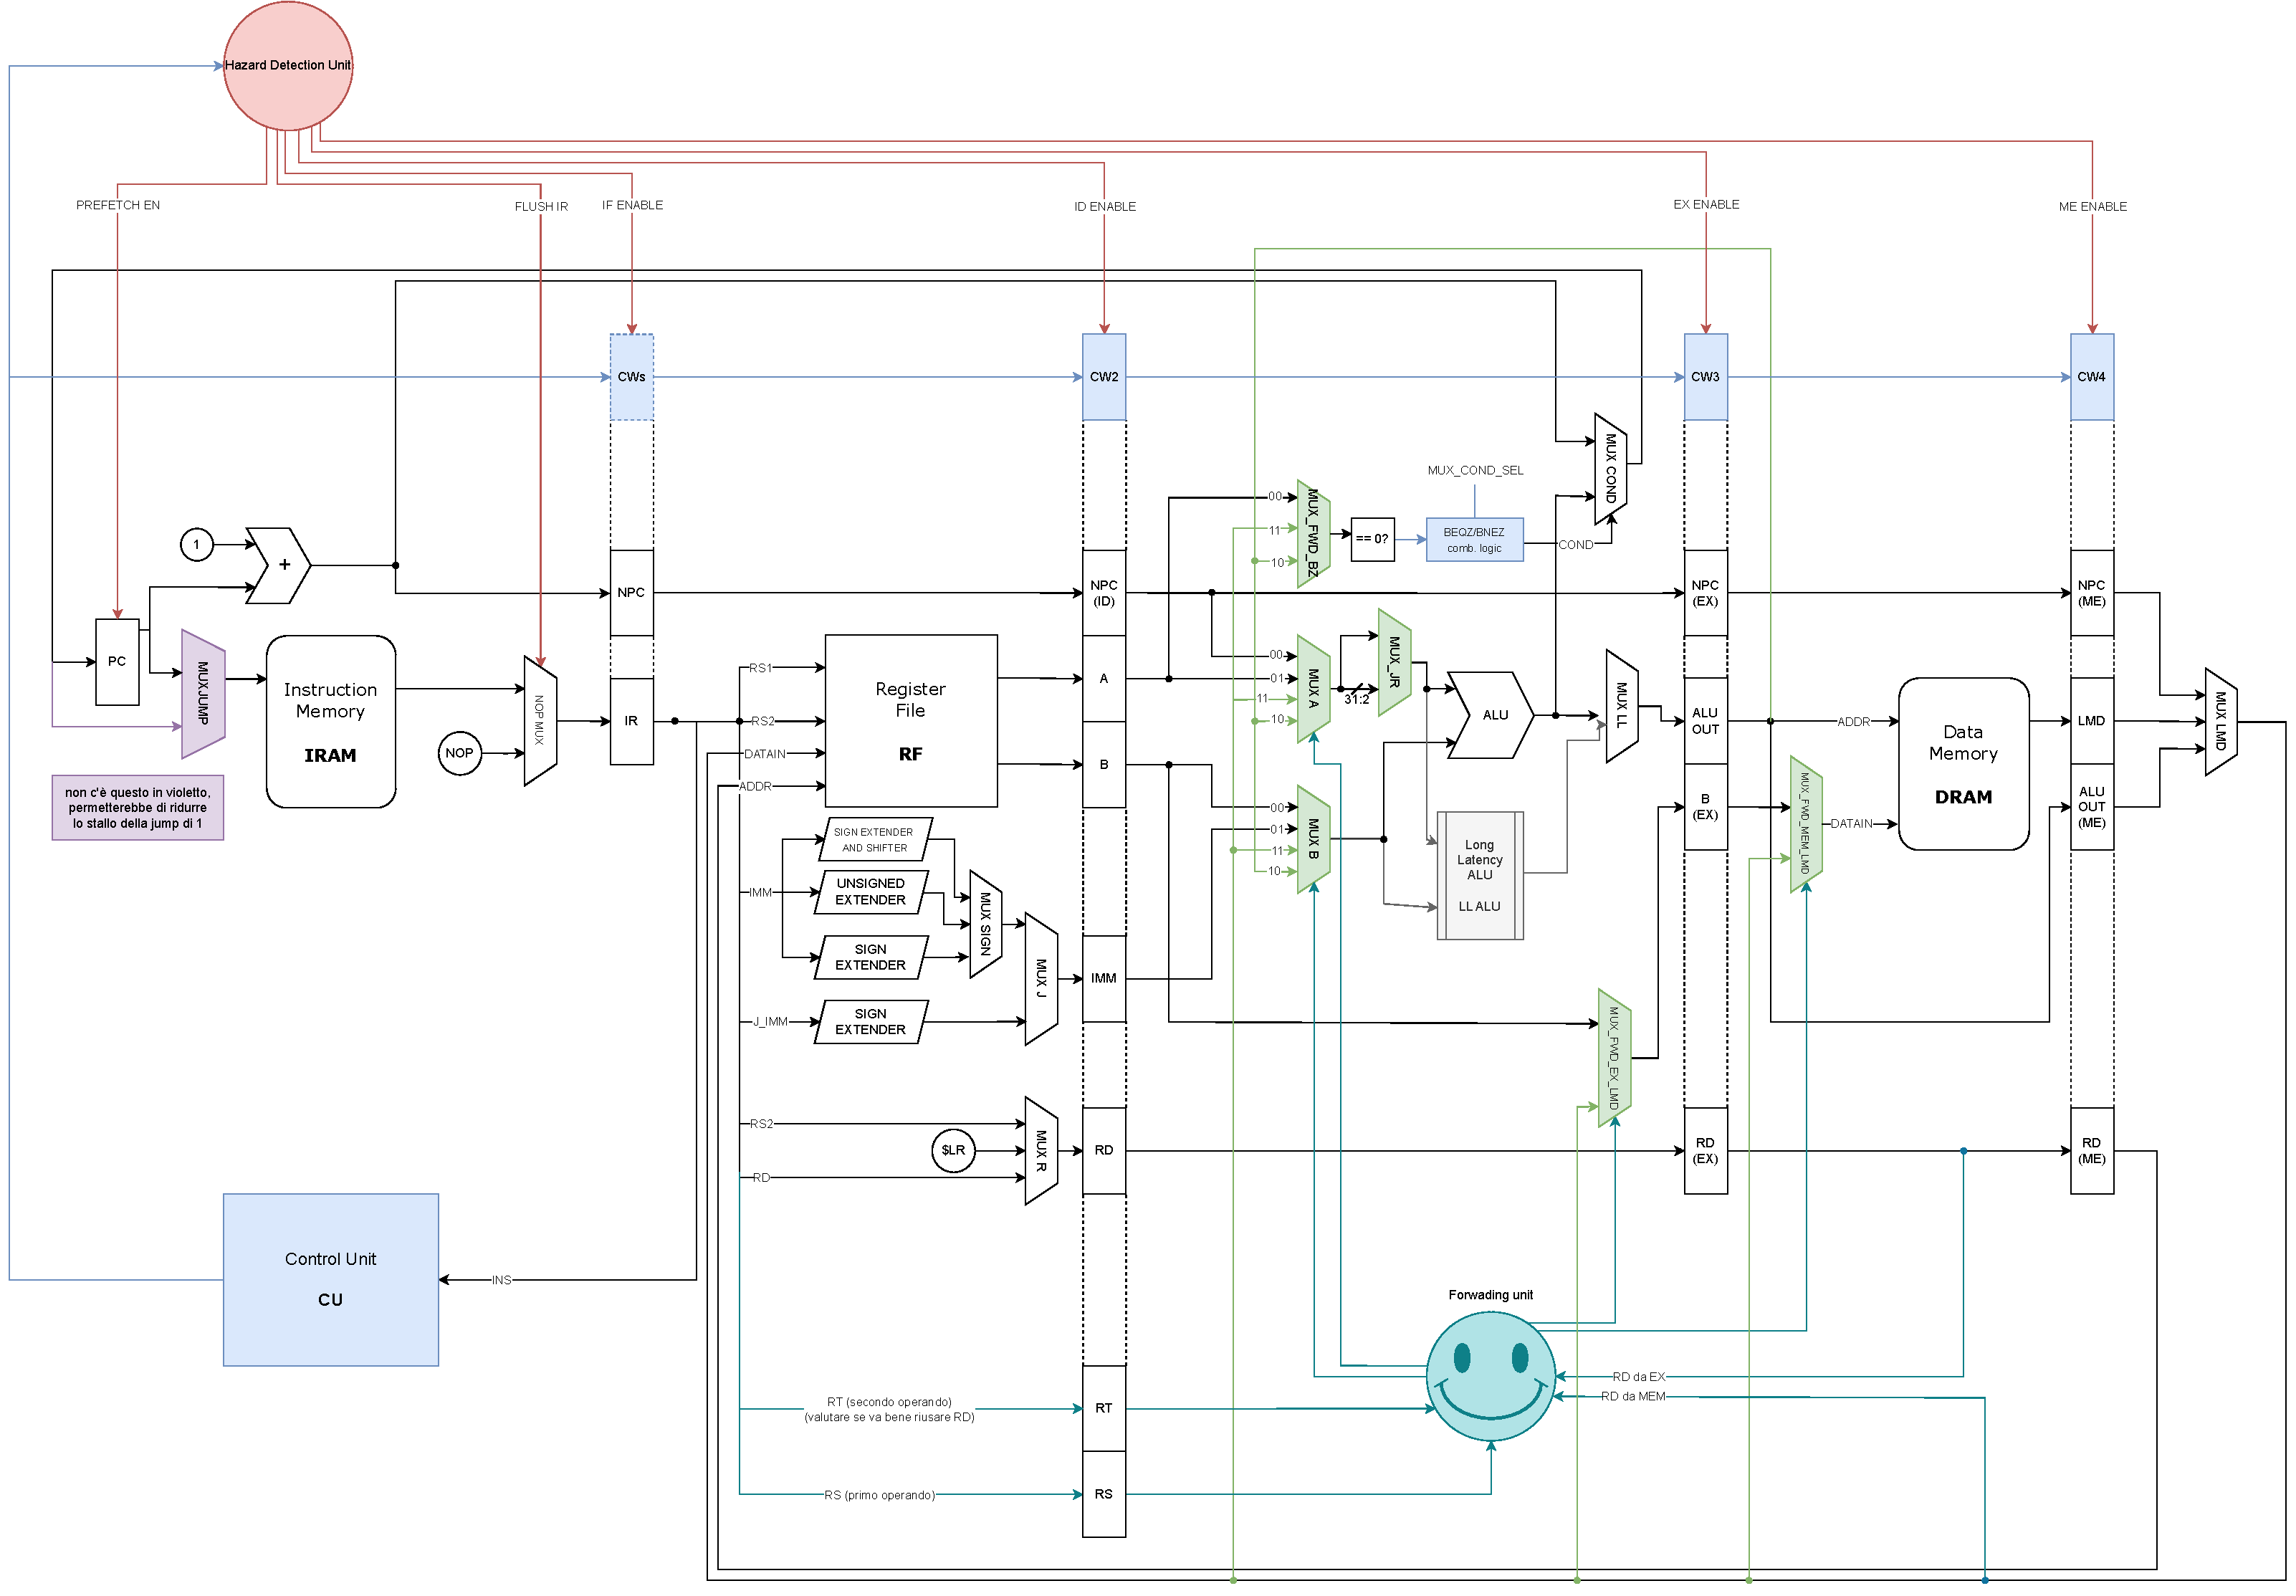
\includegraphics[width=\textwidth]{chapters/figures/datapath.pdf} 
	\caption{sus}
	\label{fig:datapath}
\end{figure}


% sezione sulle singole unità funzionali del datapath, presentate come blackbox e successivamente con l'implementazione interna, questo per ognuna di esse
\section{Functional blocks}
\subsection{Control unit}
% TODO schema della control unit? si dovrebbe vedere come viene effettivamente sintetizzata
% CHE CAZZO È CW_FROM_MEM DIO CANE
The Control Unit is in charge of managing the datapath throughout its stages. Given an instruction from IR, it generates the corresponding control word that manages the various registers, MUXes and other control signals in the datapath. It also receives a block of \emph{STALL} signals from the HDU (Hazard Detection Unit) that instructs the CU on when to stall the pipeline in case of data hazards. % solo data hazards?



% non so se questa cosa è effettivamente vera, è una LUT alla fine
It is implemented as an hybrid between an hardwired and a microcoded CU, with two processes that simply associate every instruction with a given control word and every ALU opcode with the corresponding operation, plus a process that manages the transition between every stage taking into consideration the \emph{STALL} signals from the HDU.

\subsection{Register file}
\subsection{ALU}
% TODO aggiungere schema a blocchi dell'ALU
% scrivi anche come sono mussati gli ingressi
% The ALU can pick its inputs from a moltitude of sources 
The ALU of the DLX operates on two inputs: \emph{DATA1} and \emph{DATA2}. It can obtain them from a multitude of sources, namely: 
\begin{itemize}
	% Gli input muxati possono essere non solo i registri di ingresso A e B ma anche forwardati da altri stage, essere un immediato etc.
	\item from the register file, through 2 stage registers \emph{A} and \emph{B};
	\item from the program counter, necessary for address computations in branching and jump instructions;
	\item from the instructions themselves, immediate values via the instruction register after the appropriate transformations;
	\item from the ALU itself, and in general from other stages' outputs through MUXes controlled by the forwarding unit.
\end{itemize}
% La grandezza è configurabile ma è settata di default a 32 bits IIRC


The function to be computed on the operands is selected by a third input \emph{FUNC} that receives a code representing it and the result is sent to the output \emph{OUTALU}. A list of currently implemented functions follows. The implementation of each operation is behavioural unless specified otherwise. 

% TODO fix indentations
\subsubsection{Addition}
$ \mathit{ALUOUT} = \mathit{DATA1} + \mathit{DATA2} $

A P4 adder is present inside the ALU to perform additions. Further details on its implementation together with the VHDL description are included in lab 2's zip file.

\subsubsection{Subtraction}
$ \mathit{ALUOUT} = \mathit{DATA1} - \mathit{DATA2} $


The P4 adder is also used for subtractions, by means of negating one of  the inputs and setting the carry-in input of the adder to 1.

\subsubsection{Multiplication}
% TODO aggiungere simbolo del troncamento a word size
$ \mathit{ALUOUT} = \mathit{DATA1} \cdot \mathit{DATA2} $


Multiplication is executed on the operands fully but the result is still word size: the most significant half of the computed value is discarded.


Initially, the multiplication operation was to be delegated to a long latency ALU, with this implementation just being a placeholder. However the group decided to focus on more difficult to implement features, leaving no time for description and testing of an LL ALU.

\subsubsection{AND}
$ \mathit{ALUOUT} = \mathit{DATA1} \wedge \mathit{DATA2} $

\subsubsection{OR}
$ \mathit{ALUOUT} = \mathit{DATA1} \lor \mathit{DATA2} $

\subsubsection{XOR}
$ \mathit{ALUOUT} = \mathit{DATA1} \oplus \mathit{DATA2} $

\subsubsection{Logical Shift Left}
$ \mathit{ALUOUT} = \mathit{DATA1} \ll \mathit{DATA2} $

\subsubsection{Logical Shift Right}
$ \mathit{ALUOUT} = \mathit{DATA1} \gg \mathit{DATA2} $

\subsubsection{Set equal}
$ \mathit{if (DATA1 == DATA2) \: then} \: \mathit{ALUOUT} = 1 \: \mathit{else} \: 0 $

\subsubsection{Set not equal}
$ \mathit{if (DATA1 \neq DATA2) \: then} \: \mathit{ALUOUT} = 1 \: \mathit{else} \: 0 $

\subsubsection{Set greater than or Equal (signed and unsigned)}
$ \mathit{if (DATA1 \geq DATA2) \: then} \: \mathit{ALUOUT} = 1 \: \mathit{else} \: 0 $

\subsubsection{Set greater than (signed and unsigned)}
$ \mathit{if (DATA1 > DATA2) \: then} \: \mathit{ALUOUT} = 1 \: \mathit{else} \: 0 $

\subsubsection{Set less than or Equal (signed and unsigned)}
$ \mathit{if (DATA1 \leq DATA2) \: then} \: \mathit{ALUOUT} = 1 \: \mathit{else} \: 0 $

\subsubsection{Set less than (signed and unsigned)}
$ \mathit{if (DATA1 < DATA2) \: then} \: \mathit{ALUOUT} = 1 \: \mathit{else} \: 0 $

\subsection{Hazard detection unit}
The Hazard Detection Unit takes care of detecting data and control hazards in the pipeline and successively dispatching stage enable (or STALL, as written in the CU subsection) signals to the CU for indication on where and for how many stages to stall for. It does so by progressively checking for hazardous conditions in a process starting from IRAM and DRAM readiness, then for branches (assuming not taken), jumps and loads from memory giving precedence, in case of instructions of the same type, to instructions currently found in the execute stage. If no hazardous condition is found, a STALL\_CLEAR signal is sent out.

\subsection{Forwarding unit}
The Forwarding Unit takes as input a subset of the control signals sent by the CU and of the register selection codes (not the values inside the registers themselves). Given those, it detects favourable conditions for source and destination registers between stages of the pipeline and if they match it forwards operands where they are needed by changing selection signals for the appropriate MUXes and skipping the write-back stage.
% \input{./chapters/chap_name}
% and so on
%
%%%%%%%%%%%%%%%%%%%%%%%%%%%%%%%%%%%%%%%%%%%%%%%%%%%%%%
%    
% HERE IS WHERE YOU INCLUDE YOUR APPENDICES (IF ANY)
%
\appendix
%%%% Appendix A
\chapter{Adder behavioural VHDL}
\label{appendix1}

	\lstinputlisting[language=VHDL, breaklines=true]{appendices/files/adder.vhd}

% \lstinputlisting is an alternative way to import text or code from an external file. In this example the behavioural VHDL description of an adder contained in the file adder.vhd is imported. 
% Note that you can set the language of the code that you want to import (VHDL in this example). When you set the language you will see the keywords of that specific language highlighted in your output pdf file.
%You can set a lot parameters: for some examples take a look at the chapter 'How to document the project' that can you find in DLX_Project.pdf.
% \input{./appendices/appendix2}
% and so on
%
%%%%%%%%%%%%%%%%%%%%%%%%%%%%%%%%%%%%%%%%%%%%%%%%%%%%%%

\end{document}